%% LyX 2.3.5.2 created this file.  For more info, see http://www.lyx.org/.
%% Do not edit unless you really know what you are doing.
\documentclass[letterpaper,oneside,spanish]{book}
\PassOptionsToPackage{vlined,linesnumbered,ruled}{algorithm2e}
\usepackage[T1]{fontenc}
\usepackage[utf8]{inputenc}
\setcounter{secnumdepth}{3}
\usepackage{pifont}
\usepackage{algorithm2e}
\usepackage{amsmath}
\usepackage{amsthm}
\usepackage{graphicx}

\makeatletter

%%%%%%%%%%%%%%%%%%%%%%%%%%%%%% LyX specific LaTeX commands.
\pdfpageheight\paperheight
\pdfpagewidth\paperwidth


%%%%%%%%%%%%%%%%%%%%%%%%%%%%%% User specified LaTeX commands.
\usepackage{indentfirst}

\usepackage{titlesec}
\titleformat{\chapter}[display]{\bfseries\centering\larger}{\normalsize{\chaptertitlename\ \thechapter}}{0.5ex}{}[]
\titlespacing*{\chapter}{0pt}{-50pt}{20pt}
\titleformat{\section}[hang]{\bfseries\normalsize}{\thesection\ }{0pt}{}[]
\titleformat{\subsection}[runin]{\bfseries\normalsize}{\thesubsection\ }{0pt}{}[]
\titleformat{\paragraph}[runin]{\itshape\normalsize}{\theparagraph\ }{0pt}{}[]

\newtheoremstyle{myplain}{\topsep}{\topsep}{\itshape}{}{\scshape}{.}{.5em}{}
\newtheoremstyle{mydef}{\topsep}{\topsep}{\normalfont}{}{\scshape}{.}{.5em}{}
\theoremstyle{myplain}
\newtheorem{mythm}{Teorema}[]
\newtheorem{mylem}{Lema}[]
\newtheorem{myprop}{Proposición}[]
\theoremstyle{mydef}
\newtheorem{mydef}{Definición}[]
\newtheorem{myrmk}{Observación}[]
\newtheorem{myex}{Ejemplo}[]

\let\thm\mythm
\let\endthm\endmythm
\let\lem\mylem
\let\endlem\endmylem
\let\prop\myprop
\let\endprop\endmyprop
\let\defn\mydef
\let\enddefn\endmydef
\let\example\myex
\let\endexample\endmyex
\let\rem\myrmk
\let\endrem\endmyrmk

\usepackage{xpatch}
\newcommand{\proofnamefont}{\scshape}
\xpatchcmd{\proof}{\itshape}{\normalfont\proofnamefont}{}{}

\AtBeginDocument{
  \def\labelitemi{\Pisymbol{psy}{183}}
  \def\labelitemii{\Pisymbol{psy}{45}}
  \def\labelitemiii{\Pisymbol{psy}{215}}
}

\makeatother

\usepackage{babel}
\addto\shorthandsspanish{\spanishdeactivate{~<>.}}

\begin{document}

\chapter*{Análisis de la Exactitud de un Algoritmo}

El primer paso al analizar un algoritmo es determinar si éste es correcto
o incorrecto. El procedimiento que se sigue para llevar a cabo esta
tarea se denomina \emph{análisis de la exactitud} \emph{de un algoritmo}
(o, simplemente, \emph{análisis de exactitud}).

\section*{Demostrando que un algoritmo es incorrecto}

Para demostrar que un algoritmo es incorrecto basta con producir un
\emph{contraejemplo}; esto es, un caso específico para el cual el
algoritmo no genera un resultado que satisfaga los requerimientos
de salida del problema o no termina su ejecución. Un buen contraejemplo
debe tener las sig. características:
\begin{itemize}
\item \emph{Verificabilidad}: debe ser posible determinar el resultado que
el algoritmo producirá para el contraejemplo propuesto. También debe
ser posible determinar el resultado correcto que el algoritmo debió
haber producido. 
\item \emph{Simplicidad}: el contraejemplo debe exponer claramente porqué
el algoritmo es incorrecto, sin recurrir a detalles innecesarios.
Una vez que se encuentra un contraejemplo, se recomienda simplificarlo
a su forma más básica.
\end{itemize}
Algunos consejos para encontrar buenos contraejemplos:
\begin{itemize}
\item Proponer casos específicos de tamaño lo más pequeño posible. Esto
va de la mano con el concepto de simplicidad mencionado anteriormente.
\item Considerar todas las posibles \emph{clases de entrada}; esto es, las
diferentes formas en las que pueden presentarse los casos específicos.
Por ejemplo, si la entrada de un algoritmo son dos conjuntos, entonces
se tienen cuatro clases de entrada diferentes: dos conjuntos disjuntos,
dos conjuntos que se intersectan, un subconjunto propio del otro o
dos conjuntos iguales.
\item Proponer casos específicos con valores de frontera. Esto es, tomar
los casos específicos más extremos que admite el algoritmo y observar
cómo se comporta.
\item En cuanto a algoritmos voraces,\emph{ }proponer casos específicos
cuyos elementos sean todos del mismo valor. Esto va de la mano con
el punto anterior y se refiere a observar cómo se comporta el algoritmo
en caso de empates.
\end{itemize}
En caso de no haberse encontrado un contraejemplo para un algoritmo
determinado, esto no implica que dicho algoritmo es correcto; aún
es necesario presentar una demostración convincente de su exactitud.

\section*{La invariante de lazo}

Una invariante de lazo es una proposición lógica que se cumple inmediatamente
antes e inmediatamente después de la ejecución de cada iteración de
un bucle. Algunos consejos para elegir una buena invariante de lazo
son:
\begin{itemize}
\item Comenzar por realizar una ``prueba de escritorio'' del algoritmo.
Esto ayuda a entender mejor cómo funciona y a encontrar patrones en
su comportamiento que podrían utilizarse para definir una invariante
de lazo.
\item Al trabajar con arreglos, la invariante de lazo suele mostrar alguna
característica particular de los elementos que han sido procesados
hasta el momento.
\item Al trabajar con valores numéricos, la invariante de lazo suele describir
alguna relación matemática entre ellos.
\item La invariante de lazo se debe definir en función del número de iteraciones
ejecutadas hasta el momento. 
\end{itemize}
Demostrar que una invariante de lazo se cumple para cualquier iteración
es un procedimiento análogo a una demostración por inducción y consiste
de las sig. etapas: 
\begin{enumerate}
\item \emph{Inicialización}: se considera cuál es el estado del algoritmo
que se tiene antes de comenzar a ejecutar la primera iteración\emph{
}del bucle y se procede a demostrar que la invariante de lazo se cumple
bajo estas condiciones.
\item \emph{Mantenimiento}: se hace la suposición de que la invariante de
lazo se cumple antes de comenzar alguna iteración genérica $i$ y
se determina el estado del algoritmo que se obtiene como consecuencia
de ello. Después, partiendo de dicho estado, se ejecuta una iteración
del bucle y, de nuevo, se determina el estado del algoritmo que se
obtuvo como resultado. Finalmente, partiendo de dicho estado, se procede
a demostrar que la invariante de lazo se cumple antes de comenzar
la iteración $i+1$.
\item \emph{Finalización}: se determina cuál es el estado del algoritmo
cuando el bucle termina su ejecución y, partiendo de dicho estado,
se procede a utilizar la invariante de lazo para demostrar que el
algoritmo es correcto o para demostrar que se cumple alguna propiedad
particular del algoritmo. 
\end{enumerate}

\section*{Consejos para diseñar algoritmos correctos}

Cuando se trata de diseñar algoritmos, rara vez es posible producir
uno que sea correcto al primer intento; normalmente, el diseño de
un algoritmo es un proceso iterativo. A continuación se presentan
algunos consejos que pueden facilitar la tarea de diseñar algoritmos
correctos. 

\subsection*{Definición del problema}

El primer paso para diseñar un algoritmo correcto es definir claramente
los requerimientos de entrada y salida del problema a resolver. Si
el problema está mal definido, el algoritmo será incorrecto sin importar
lo que se haga. Algunos consejos para definir correctamente el problema
son:
\begin{itemize}
\item De ser posible, se recomienda hacer más específicos los requerimientos
de entrada; esto suele reducir la dificultad para resolver el problema.
Por ejemplo, intentar trabajar con árboles en lugar de grafos generales.
\item Se debe ser explícito con los requerimientos de salida. Por ejemplo,
en lugar de simplemente pedir la ``mejor'' trayectoria entre dos
lugares en el mapa, es preferible pedir la ruta de menor distancia
o la que requiera la menor cantidad de giros a la izquierda.
\item Los requerimientos de salida deben ser simples. Por ejemplo, ``encontrar
la ruta más corta entre dos lugares en el mapa que no requiera más
del doble de giros a la izquierda de los que son necesarios'' es
una salida bien definida pero muy complicada de satisfacer puesto
que está compuesta de tres objetivos más específicos. 
\end{itemize}

\subsection*{Abordar el problema por dos ángulos}

Al trabajar con problemas nuevos, se recomienda estudiar la complejidad
computacional del problema al mismo tiempo que se diseña un algoritmo
para resolverlo. De esta forma, cualquier avance o descubrimiento
que se obtenga al estudiar la complejidad puede utilizarse después
para avanzar el diseño del algoritmo y vice versa. Además, al final
se obtendrá uno de dos posibles resultados: ya sea se demuestra la
complejidad del problema o se llega a la construcción de un nuevo
algoritmo para resolverlo. 

\subsection*{Selección de una estructuras abstracta}

Casi cualquier problema, aplicación o sistema en la vida real se puede
formular en términos de alguna \emph{estructura abstracta} y de sus
operaciones fundamentales. Como consecuencia, muchos problemas se
pueden resolver aprovechando algoritmos y estructuras de datos ya
conocidos. Sin embargo, las especificaciones del problema no siempre
se ajustarán perfectamente a las características de la estructura
elegida. En estos casos, se recomienda ignorar temporalmente aquellos
detalles que no encajen y decidir más adelante, después de trabajar
un tiempo con esa estructura, si dichos detalles son realmente esenciales
o no para resolver el problema. 

A continuación se presenta una lista de las estructuras abstractas
más comunes. Cabe señalar que todas estas estructuras son \emph{recursivas};
esto es, se pueden descomponer en estructuras más pequeñas pero de
propiedades idénticas a la original. 
\begin{itemize}
\item \emph{Permutaciones}: representan diferentes ordenamientos de una
misma secuencia de objetos. Eliminando el primer elemento de una permutación
produce una permutación de menor longitud.
\item \emph{Subconjuntos}: representan colecciones de objetos seleccionados
de alguna otra colección (tal vez) más grande. Eliminando un elemento
de un subconjunto produce un subconjunto de menor cardinalidad.
\item \emph{Árboles}: representan relaciones jerárquicas entre varios objetos.
Eliminando la raíz de un árbol produce una colección de árboles con
menos nodos (denominado \emph{bosque}). Eliminando una hoja de un
árbol produce un árbol con menos nodos.
\item \emph{Grafos}: representan las relaciones entre pares arbitrarios
de objetos. Eliminando un vértice de un grafo produce un grafo con
menos vértices. Separando los vértices en dos grupos y eliminando
todas las aristas que crucen de un grupo a otro, produce dos grafos
con menos aristas.
\item \emph{Puntos}: representan diferentes posiciones en un mismo espacio
geométrico. Separando una nube de puntos en dos grupos produce dos
nubes de puntos más pequeños.
\item \emph{Polígonos}: representan diferentes regiones en un mismo espacio
plano. Conectando dos vértices no adyacentes con una recta produce
dos polígonos de menor área.
\item \emph{Cadenas}: representan diferentes secuencias de una misma colección
de símbolos. Eliminando el primer símbolo de una cadena produce una
cadena de menor longitud.
\end{itemize}
\begin{figure}[tb]
\begin{centering}
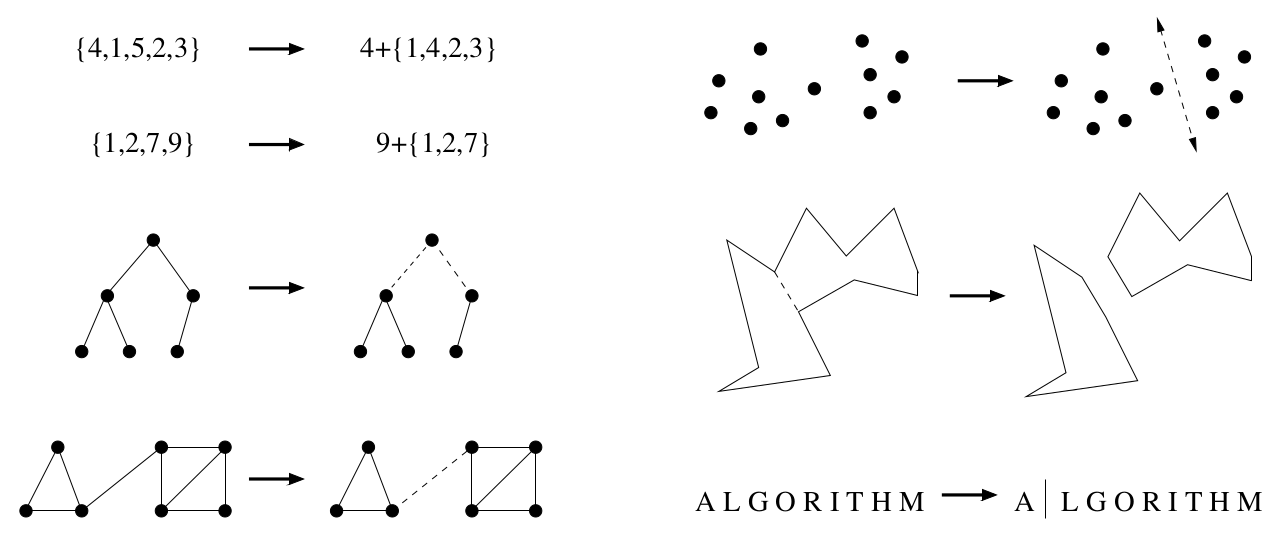
\includegraphics[width=1\textwidth]{figuras/estructuras}
\par\end{centering}
\caption{{\small{}Descomposición recursiva de algunas estructuras abstractas.
(Izquierda) Permutaciones, subconjuntos, árboles y grafos. (Derecha)
Puntos, polígonos y cadenas.}}
\end{figure}


\section*{Notas bibliográficas}
\begin{itemize}
\item Cormen T.H., Leiserson C.E., Rivest R.L. \& Stein C., ``Introduction
to Algorithms'', 3ra ed. (2009), MIT Press. Págs. 18-20. 
\item Skiena S.S., ``The Algorithm Design Manual'', 2da ed. (2012), Springer.
Págs. 11-16.
\end{itemize}

\end{document}
